	\newpage
\section{Ogólne określenie wymagań projektu}		%1
%Ogólne określenie wymagań i zakresu programu (Czyli zleceniodawca określa wymagania programu) 

\subsection{Ogólny zarys wymagań}

Celem programu jest pełnienie funkcji odtwarzacza muzyki oraz dodatkowo ma on pełnić rolę dyktafonu. Program będzie mógł skanować dany folder, a w nim tagi zawartych plików muzycznych i tworzyć na jego podstawie graficzną reprezentację biblioteki. 

\subsection{Wykorzystane czujniki}

Program ma na celu wykorzystanie trzech czujników, z którymi użytkownik będzie wchodził w interakcję. Zostaną użyte następujące:

\begin{itemize}
	\item Żyroskop - Interfejs programu będzie się zmieniał w zależności od orientacji urządzenia. 
	
	\item Mikrofon - Program będzie posiadał funkcję nagrywania dźwięku. Nagrane pliki będzie można odtwarzać w odtwarzaczu

	\item Czujnik światła - Interfejs programu będzie mógł zmieniać swoje kolory w zależności od wykrytego poziomu światła na czujniku
\end{itemize}

\subsection{Zarys interfejsu}

\begin{figure}[H]
	\centering
	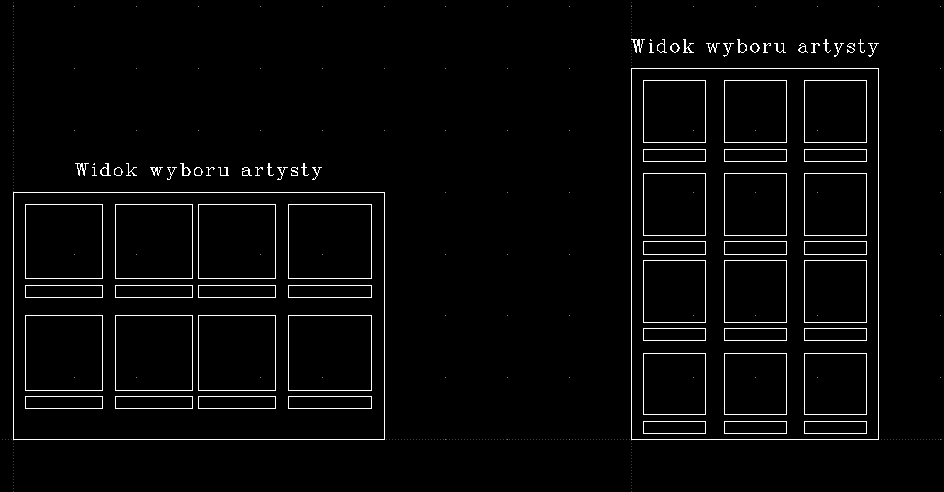
\includegraphics[width=1\textwidth]{images/mockup_artysta.png}
	\caption{\centering{Mockup widoku biblioteki - listing wykonawców}}
\end{figure}

Widok wykonawców będzie ekranem startowym aplikacji. "Kafelki" będa zdjęciami wykonawców. Klikanie na jeden z nich przejdzie do widoku albumów danego wykonawcy

\begin{figure}[H]
	\centering
	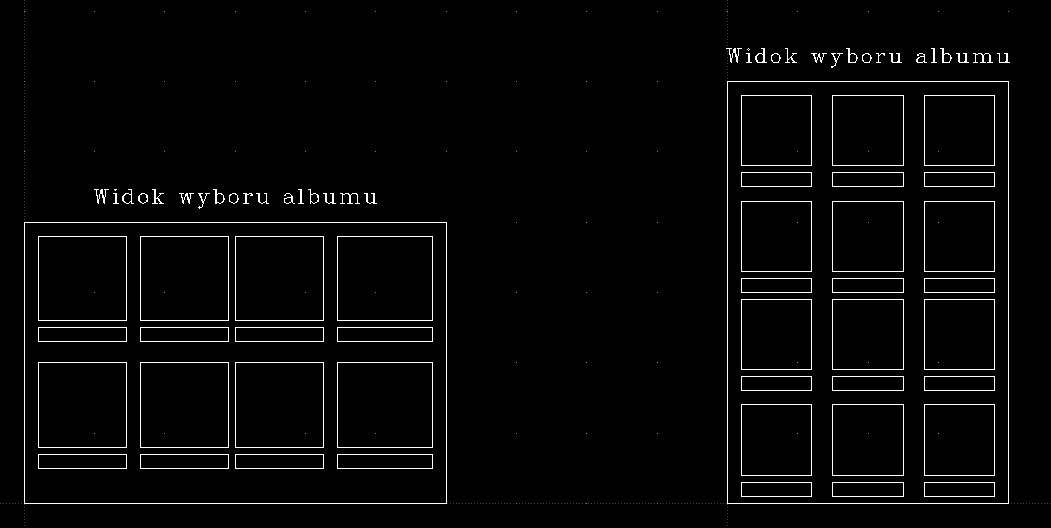
\includegraphics[width=1\textwidth]{images/mockup_albumy.png}
	\caption{\centering{Mockup widoku albumów danego wykonawcy}}
\end{figure}

Widok albumów jest identyczny jak widok wykonawców. Jedyna różnica polega tym, że zdjęcia na kafelkach będą zdjęciami albumów.

\begin{figure}[H]
	\centering
	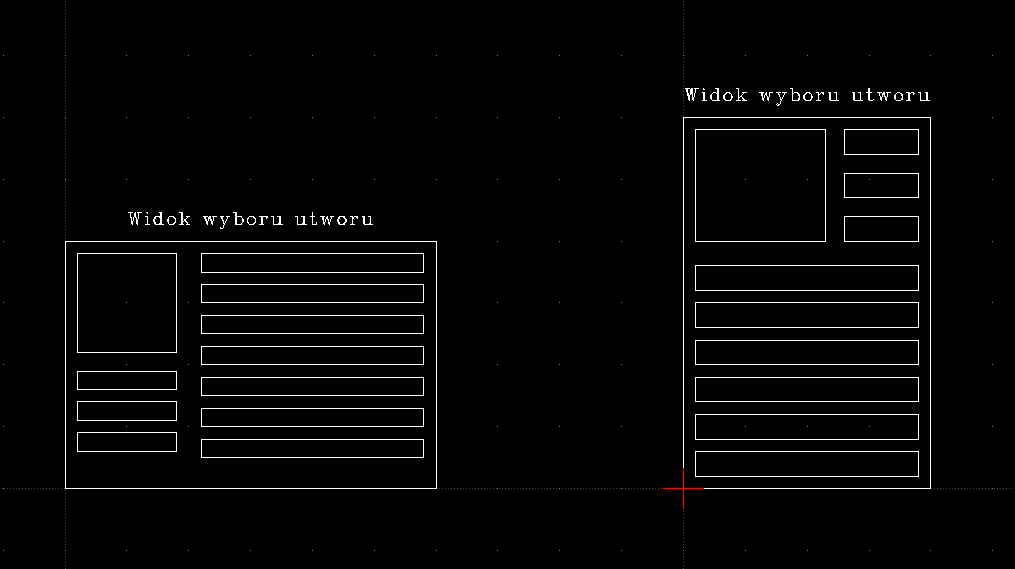
\includegraphics[width=1\textwidth]{images/mockup_utwory.png}
	\caption{\centering{Mockup widoku wyboru utworu}}
\end{figure}

Po wejściu na jakiś album zaprezentowane zostaną zawarte w nim utwory. W lewym górnym jest zdjęcie danego albumu, a obok niego jest kilka informacji o albumie jak wykonawca, data, tytuł. Dłuższe paski to lista tytułów piosenek, które można kliknąć, aby daną piosenkę włączyć.

\begin{figure}[H]
	\centering
	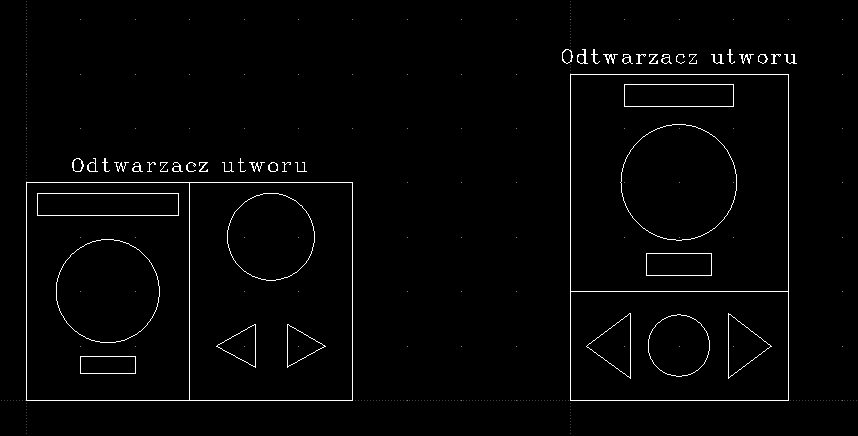
\includegraphics[width=1\textwidth]{images/mockup_odtwarzacz.png}
	\caption{\centering{Mockup odtwarzacza}}
\end{figure}

Odtwarzacz będzie działał następująco: duże koło będzie stylizowane na płytę, gdzie wypełniona ona będzie obrazem albumu. Płyta ta będzie się kręcić w czasie gdy gra piosenka. Kąt płyty (od 0\degree, do 360\degree) będzie określał jak duża część piosenki została odtworzona. Kąt ten będzie określony jeszcze niezdefiniowanym efektem graficznym. Prostokąty wokół płyty to tytuł piosenki, a na dole czas grania. Kółko i wokół niego trójkąty to przyciski odtwarzania - graj/pauza, następny, poprzedni. 

\begin{figure}[H]
	\centering
	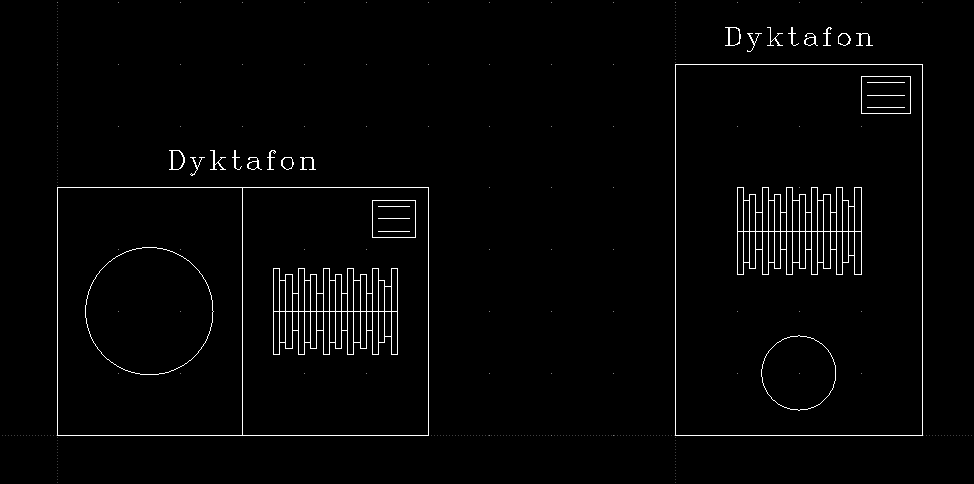
\includegraphics[width=1\textwidth]{images/mockup_dyktafon.png}
	\caption{\centering{Mockup dyktafonu}}
\end{figure}

Do dyktafonu będzie można się dostać przesuwając palcem w prawo na ekranie wykonawców. Dyktafon jest aktywowany wielkim okrągłym przyciskiem. Te kreski obok niego to wizualizacja dźwięku z mikrofonu. Menu w rogu będzie pozwalało na m.in. skonfigurowanie folderu zapisu nagrań.
